\chapter{Coulomb scattering}
\label{Coulomb scattering}

\section{Leading order calculation}

We consider in this section the scattering of an electron by an atomic nucleus of atomic number $Z$.
We model the nucleus by a classical point charge without magnetic moment, being at rest at the origin in the lattice reference frame and having a mass much higher than the mass of the electron.
The corresponding electromagnetic field is described as a classical Coulomb potential $\V^{cl}$ given in terms of Fourier components by:
\begin{eqnarray*}
\V^{cl}_{\n} & \eqdef & ( 1 + 2 \N )^{-3} \sum_{\q_\photon \neq \sv 0} \FT \V^{cl}_{\q_\photon} \exp{\i 2 \pi \n \ssp \q_\photon} \\
\FT \V^{cl}_{\q_\photon} & \eqdef & \frac{Z \e}{4 \pi^2 \vpty \a q_\photon^2}
\end{eqnarray*}
The corresponding semi-classical interaction Hamiltonian takes the form:
\begin{eqnarray*}
\Hop' & \eqdef & \HopQED + \Hop^{cl} \\
\Hop^{cl} & \eqdef & \sum_{\n} \Qop \n \V^{cl}_{\n}
\end{eqnarray*}
and its development on the plane wave basis is given by:
\begin{eqnarray*}
\Hop^{cl} & = & \frac{Z \e^2}{4 \pi^2 \vpty \a} ( 1 + 2 \N )^{-3} \sum_{\pt, \q, \sp', \sp} \Qp \pt \sum_{\q_\photon \neq \sv 0} q_\photon^{-2} \\
&& \left( \SCop \pt {\q + \q_\photon} {\sp'} + \SAop {\antiparticle \pt} {-\q - \q_\photon} {\sp'} \right) \gammat 0 \left( \SAop \pt \q \sp + \SCop {\antiparticle \pt} {-\q} \sp \right)
\end{eqnarray*}

As initial and final states, we take:
\begin{eqnarray*}
\ket{\Psi_i} & \eqdef & \ketX 1 \electron {\q_i} {\sp_i} \\
\ket{\Psi_f} & \eqdef & \ketX 1 \electron {\q_f} {\sp_f}
\end{eqnarray*}
The matrix element of the interaction Hamiltonian is given for $\q_f \neq \q_i$ by:
\begin{equation*}
H'_{f,i} = (1 + 2 \N )^{-3} \frac {-Z \e^2}{4 \pi^2 \vpty \a \norm{\q_f - \q_i}^2} \ddirspin \electron {\q_f} {\sp_f} \dirspin \electron {\q_i} {\sp_i}
\end{equation*}
and the leading order transition probability for this process is also represented by following diagram:
\begin{center}
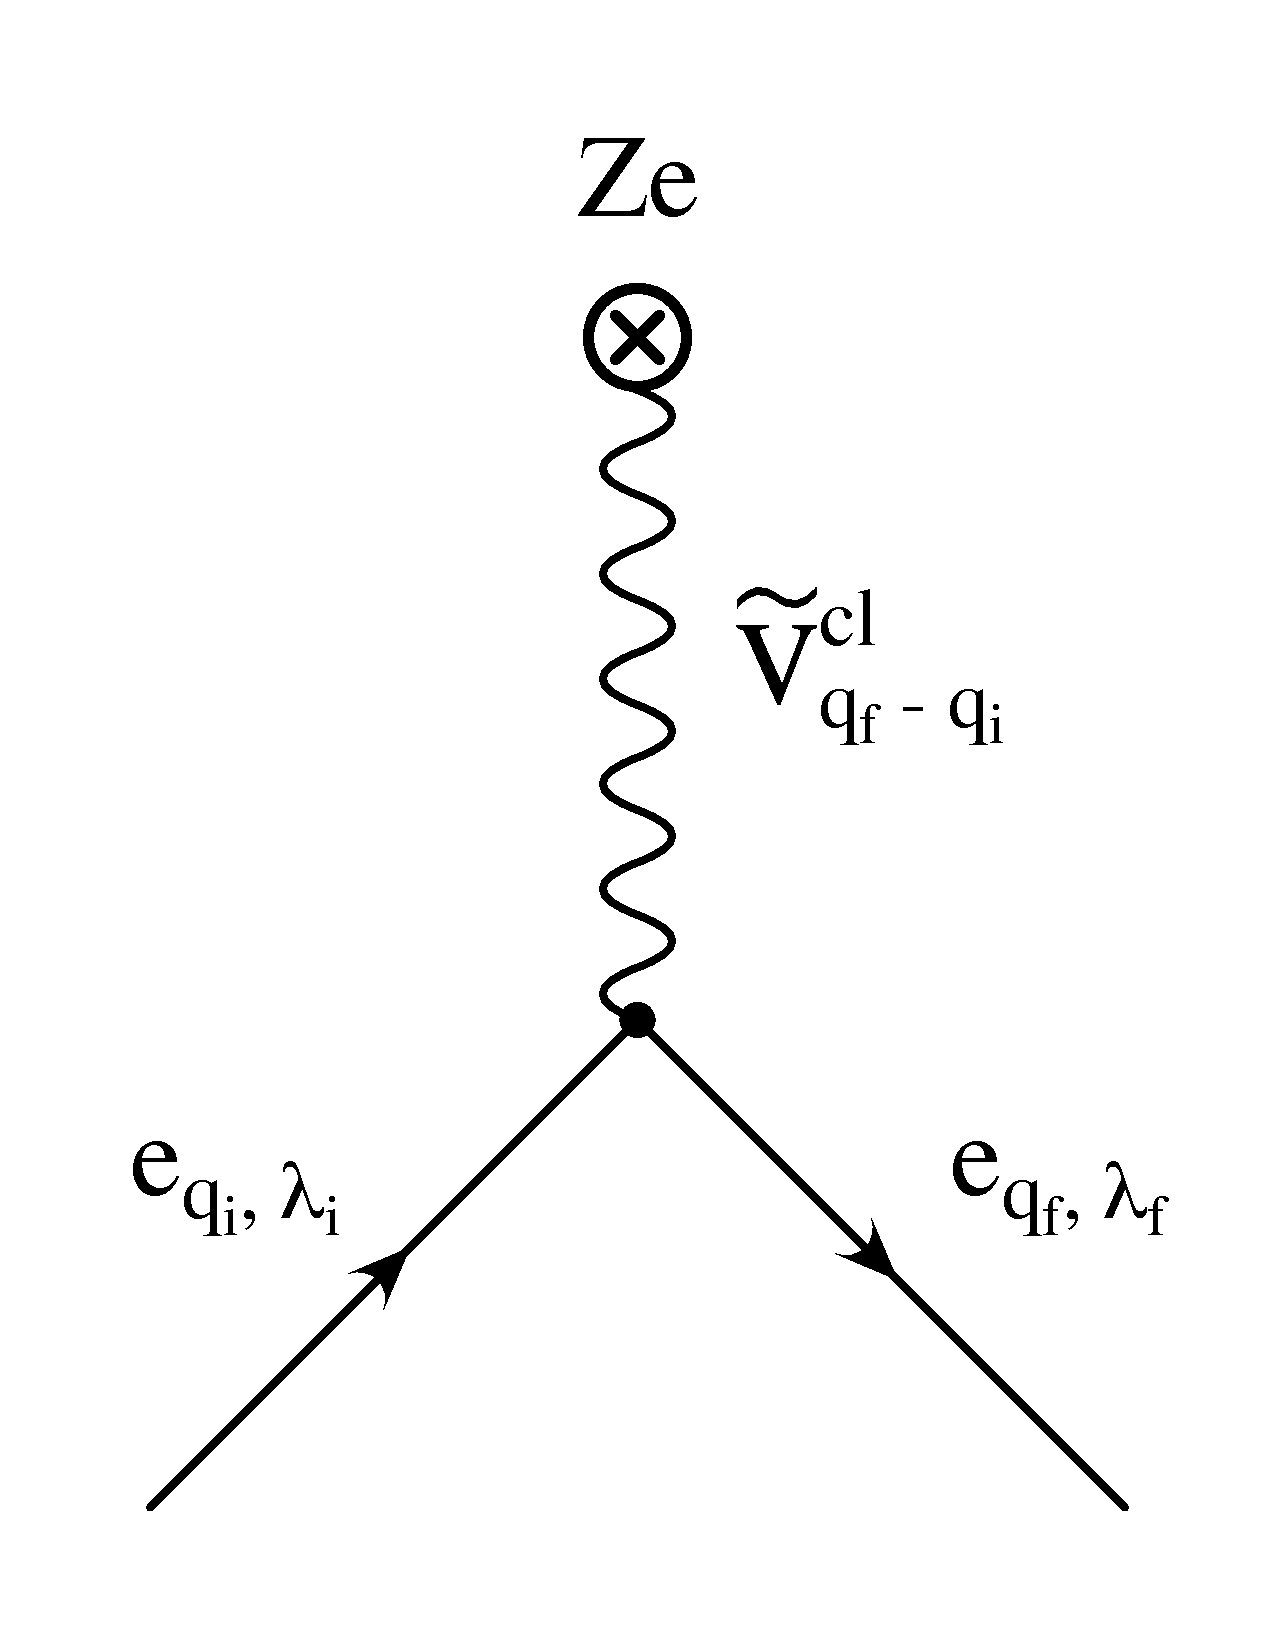
\includegraphics[scale=0.2]{images/diagrams/Coulomb_Scattering.pdf}
\end{center}
We consider a detector capturing the electrons having their momentum in the solid angle $\delta \Omega$.
For $i \notin \delta \F$, the leading order transition probability takes the form:
\begin{eqnarray*}
\TPn i {\delta \F} 2 & \approx & \int_{\delta \Omega} \int_0^{\infty} ( 2 \pi )^2 \frac{t - t_0} \h \left| H'_{f + \delta \q,i} \right|^2 \deltaE2{E_{f + \delta \q} - E_i} \\
&& \left( (1 + 2 \N) \frac \a \h \right)^3 p^2 \dnp \dO
\end{eqnarray*}
By taking following continuation for the factors of the integrand:
\begin{eqnarray*}
\left| H'_{f + \delta \q,i} \right|^2 & \approx & \left( (1+2\N) \a \right)^{-6} \frac {Z^2 \e^4 \h^4}{16 \pi^4 \vpty^2 \norm{\p - \p_i}^4} \left| \ddirspin \electron \q {\sp_f} \dirspin \electron {\q_i} {\sp_i} \right|^2 \\
\deltaE2{E_{f + \delta \q} - E_i} & \approx & \deltaE2{\sqrt{(\mp \electron \c^2)^2 + (p \c)^2} - E_i}
\end{eqnarray*}
the integration over $p$ yields to:
\begin{equation*}
\TPn i {\delta \F} 2 \approx (t - t_0) j_i \CSn i {\delta \F} 2
\end{equation*}
where $\sv j_i$ is the incident particle flux, given by:
\begin{eqnarray*}
\sv j_i & \eqdef & \left( (1+2\N) \a \right)^{-3} \sv v_i \\
\sv v_i & \eqdef & \frac {\p_i} {E_i / \c^2}
\end{eqnarray*}
and $\CSn i {\delta \F} 2$ the leading order cross section, given for $i \notin \delta \F$ by:
\begin{equation*}
\CSn i {\delta \F} 2 \approx \int_{\delta \Omega} \left( \frac {Z \e^2} {8 \pi \vpty v_i p_i} \right)^2 \left| \ddirspin \electron \q {\sp_f} \dirspin \electron {\q_i} {\sp_i} \right|^2 \frac {\dO} {\sin{\theta / 2}^4}
\end{equation*}
where $\theta$ is the deviation angle of the electron.

If the incident electron beam isn't polarized and if the polarization of the scattered electron isn't being measured, the cross section is obtained by adding the cross sections corresponding to the final spin states $\sp_f$ and averaging over the cross sections corresponding to the initial spin states $\sp_i$:
\begin{equation*}
\left< \CSn i {\delta \F} 2 \right> \approx \int_{\delta \Omega} \left( \frac {Z \e^2} {8 \pi \vpty v_i p_i} \right)^2 \frac 1 2 \sum_{\sp_f,\sp_i} \left| \ddirspin \electron \q {\sp_f} \dirspin \electron {\q_i} {\sp_i} \right|^2 \frac {\dO} {\sin{\theta / 2}^4}
\end{equation*}
The spin summation is given for $E = E_i$ by:
\begin{equation*}
\frac 1 2 \sum_{\sp_f,\sp_i} \left| \ddirspin \electron \q {\sp_f} \dirspin \electron {\q_i} {\sp_i} \right|^2 = 1 - \beta_i^2 \sin{\theta / 2}^2
\end{equation*}
and the mean cross section takes also the form:
\begin{equation*}
\left< \CSn i {\delta \F} 2 \right> \approx \int_{\delta \Omega} \left( \frac {Z \e^2} {8 \pi \vpty v_i p_i} \right)^2 \left( 1 - \beta_i^2 \sin{\theta / 2}^2 \right) \frac {\dO} {\sin{\theta / 2}^4}
\end{equation*}
The total mean cross section for deviation angles $\theta \geq \theta_m$ is also given by:
\begin{equation*}
\left< \CSn i \F 2 \right> \approx \left( \frac {Z \e^2} {8 \pi \vpty v_i p_i} \right)^2 \left( \frac {4 \pi} {\tan{\theta_m / 2}^2} + 8 \pi \beta_i^2 \ln{\sin{\theta_m / 2}} \right)
\end{equation*}
